%%%%%%%%%%%%%%%%%%%%%%%%%%%%%%%%%%%%%%%%%%%%%%%%%%%%%%%%%%%%%%%%%%%%%%%%
% Plantilla TFG/TFM
% Escuela Politécnica Superior de la Universidad de Alicante
% Realizado por: Jose Manuel Requena Plens
% Contacto: info@jmrplens.com / Telegram:@jmrplens
%%%%%%%%%%%%%%%%%%%%%%%%%%%%%%%%%%%%%%%%%%%%%%%%%%%%%%%%%%%%%%%%%%%%%%%%

\chapter{Introducción}
\label{cap1}

\begin{equation}
	y_{0}=\left ( \frac{L}{\pi} \right )\arccos\left ( \sqrt{\frac{\frac{1}{2(G_{1}\pm G_{12})}}{R_{in}}} \right )
	\label{eq:yo}
\end{equation}
\par A lo largo de este trabajo de final de grado se hará referencia a una gran parte de los conceptos básicos de Ingeniería de Telecomunicaciones que han sido impartidos durante el grado. Es por ello que en esta introducción se realizará un repaso de estos conceptos, términos y teorías imprescindibles para poder realizar y entender este estudio.
\\
\par Se realizará también una breve contextualización del proyecto para dar a entender la necesidad de esta tecnología de antenas para la nueva generación de comunicaciónes móviles en actual desarrollo: el 5G. 

\section{Las Telecomunicaciones}

\par Para entender el concepto de ``Telecomunicación" es importante fijarse en cómo la etimología de la palabra nos lleva hasta su raíz: \textit{comunicación}. La comunicación, en su significado más primitivo, es el proceso de intercambio de información entre dos sujetos definidos: un emisor que genera y emite esta información, y un receptor que la recibe y la procesa. Además, en el proceso de comunicación siempre se encontrará un tercer interviniente: el medio, encargado de transportar la información entre ambos sujetos. Por otro lado, queda el prefijo \textit{tele}, proveniente del griego: lejos o distancia. Se si regresa a la palabra original se puede definir el concepto de ``Telecomunicación" como: el proceso de intercambio de información a distancia, y aunque es una definición correcta, dista del concepto de ``Telecomunicaciones" que es utilizado día a día, el cual, trae consigo la incursión de la tecnología en él. Es por ello que la Real Academia Española (RAE) define el concepto de ``Telecomunicación" como: \cite{telecomunicacion2019}

\begin{quote}

\small Sistema de transmisión y recepción a distancia de señales de diversa naturaleza por medios electromagnéticos.

\end{quote}

\par En esta nueva definición incluimos un nuevo concepto imprescindible para poder adentrarse en las telecomunicaciones actuales: el electromagnetismo o la interacción entre campos eléctricos y magnéticos. Este último concepto hace que se pueda entender actualmente a las telecomunicaciones como una rama científica que estudia la transmisión de información, no entre sujetos personales como se han entendido hasta ahora, sino entre máquinas. Cualquier máquina  ahora podrá actuar como un sujeto transmisor, que podrá emitir información codificada de una manera determinada de forma que uno o más receptores sean capaces de recibir, decodificar y procesar esta información de manera automática.
\\
\par El electromagnetismo es la rama de la ciencia encargada de estudiar la interacción entre partículas cargadas con campos eléctricos y magnéticos. El conjunto de fenómenos electromagnéticos que se conocen hoy en día fueron estudiados por científicos como \textit{H.C. Ørsted}, \textit{André-Marie Ampère} o \textit{Michael Faraday} y unificados por \textit{James Clerk Maxwell} (Fig: \ref{fig:maxwell}) en su obra de 1865, \textit{A dynamical theory of the electromagnetic field} \cite{JamesClerkMaxwell1996}, donde se recogen las cuatro ecuaciones denominadas como ``Ecuaciones de Maxwell". La transmisión de la comunicación entre máquinas se realizará mediante impulsos eléctricos que, dada su naturaleza a variar con el tiempo y teniendo en cuenta la teoría electromagnética, se transformarán en impulsos magnéticos y viceversa. Estos impulsos electromagnéticos se transmitirán a través de un medio, en forma de \gls{oem}. A lo largo de los sigueintes capítulos se estudiará con más detenimiento los conceptos relacionados con las ondas y el medio.

\begin{figure}[h]
    \centering
       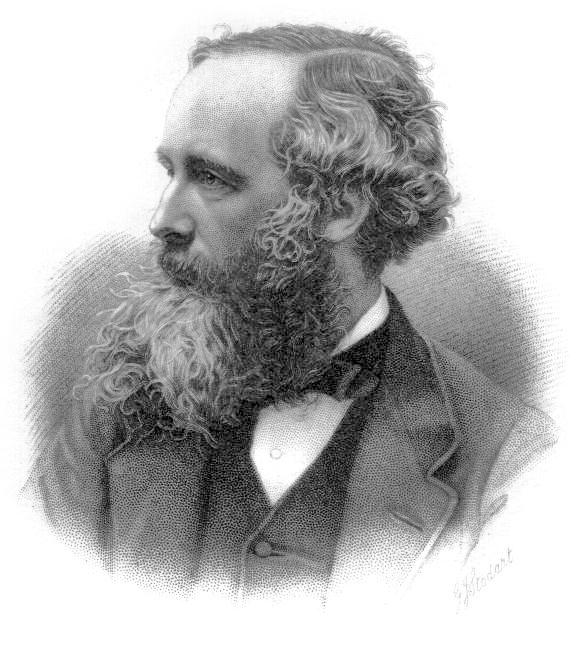
\includegraphics[width=9cm]{archivos/maxwell}
        \caption{James Clerk Maxwell (1831 - 1879). \cite{StodartCirca.1890} }
        \label{fig:maxwell}
\end{figure}

\section{Teoría de ondas y señales}
\par Como se mencionó anteriormente, en el proceso de comunicación en el ámbito de las telecomunicaciones la información se envía en forma de señales. Se consideran las señales como un conjunto de impulsos electromagnéticos transmitidos por un emisor y codificados de una manera determinada para que el o los receptores a los que vaya dirigido puedan procesar la información contenida en una señal o conjunto de ellas. Esta información transmitida en forma de señales es el mensaje.
\\
\par Una señal electromagnética se caracteriza por el hecho de variar su intensidad en el dominio temporal. El ejemplo más básico lo encontramos en la onda Seno o Coseno de la figura
\ref{fig:seno}. De esta señal es posible obtener tres parámetros básicos imprescindibles para describir cualquier otra posible señal: amplitud, frecuencia y fase. 
\\
\par Se define la amplitud como la variación máxima respecto a un origen determinado y es medido en una magnitud física concreta, en el caso mencionado, la amplitud sería de una unidad, pudiendo ser esta voltios o vatios entre otros. Al tratarse de una señal oscilante aparece el concepto de frecuencia como el número de veces que la señal vuelve a su origen en un tiempo determinado de 1 segundo, la unidad de medida de este parámetro es el \textit{hertzio} (\textbf{Hz}), para el caso mencionado, la frecuencia de la onda es de 1 Hz, puesto que en un segundo la onda realiza un ciclo completo. 
\\
\par Finalmente, se denomina fase al concepto de adelanto o retraso de la onda en el dominio temporal con respecto a un origen determinado, normalmente es representado mediante el símbolo \textit{phi} (\textbf{Φ}) y es medido en grados o radianes según sea conveniente. Para el caso mencionado la fase sería 0º, puesto que se conoce que una onda seno tiene origen en este valor y no se aprecia ningún adelanto o retraso en la onda mencionada con respecto a este. 
\\
\par Es posible agrupar estos parámetros en forma de ecuación analítica para el caso de una onda simple sin perdidas físicas ni amortiguación y con un movimiento armónico simple como:

\begin{equation}
	x(t)=A\cdot \sin(2\cdot\pi\cdot f+\phi )
	\label{eq: seno}
\end{equation}

\begin{figure}[h]
    \centering
        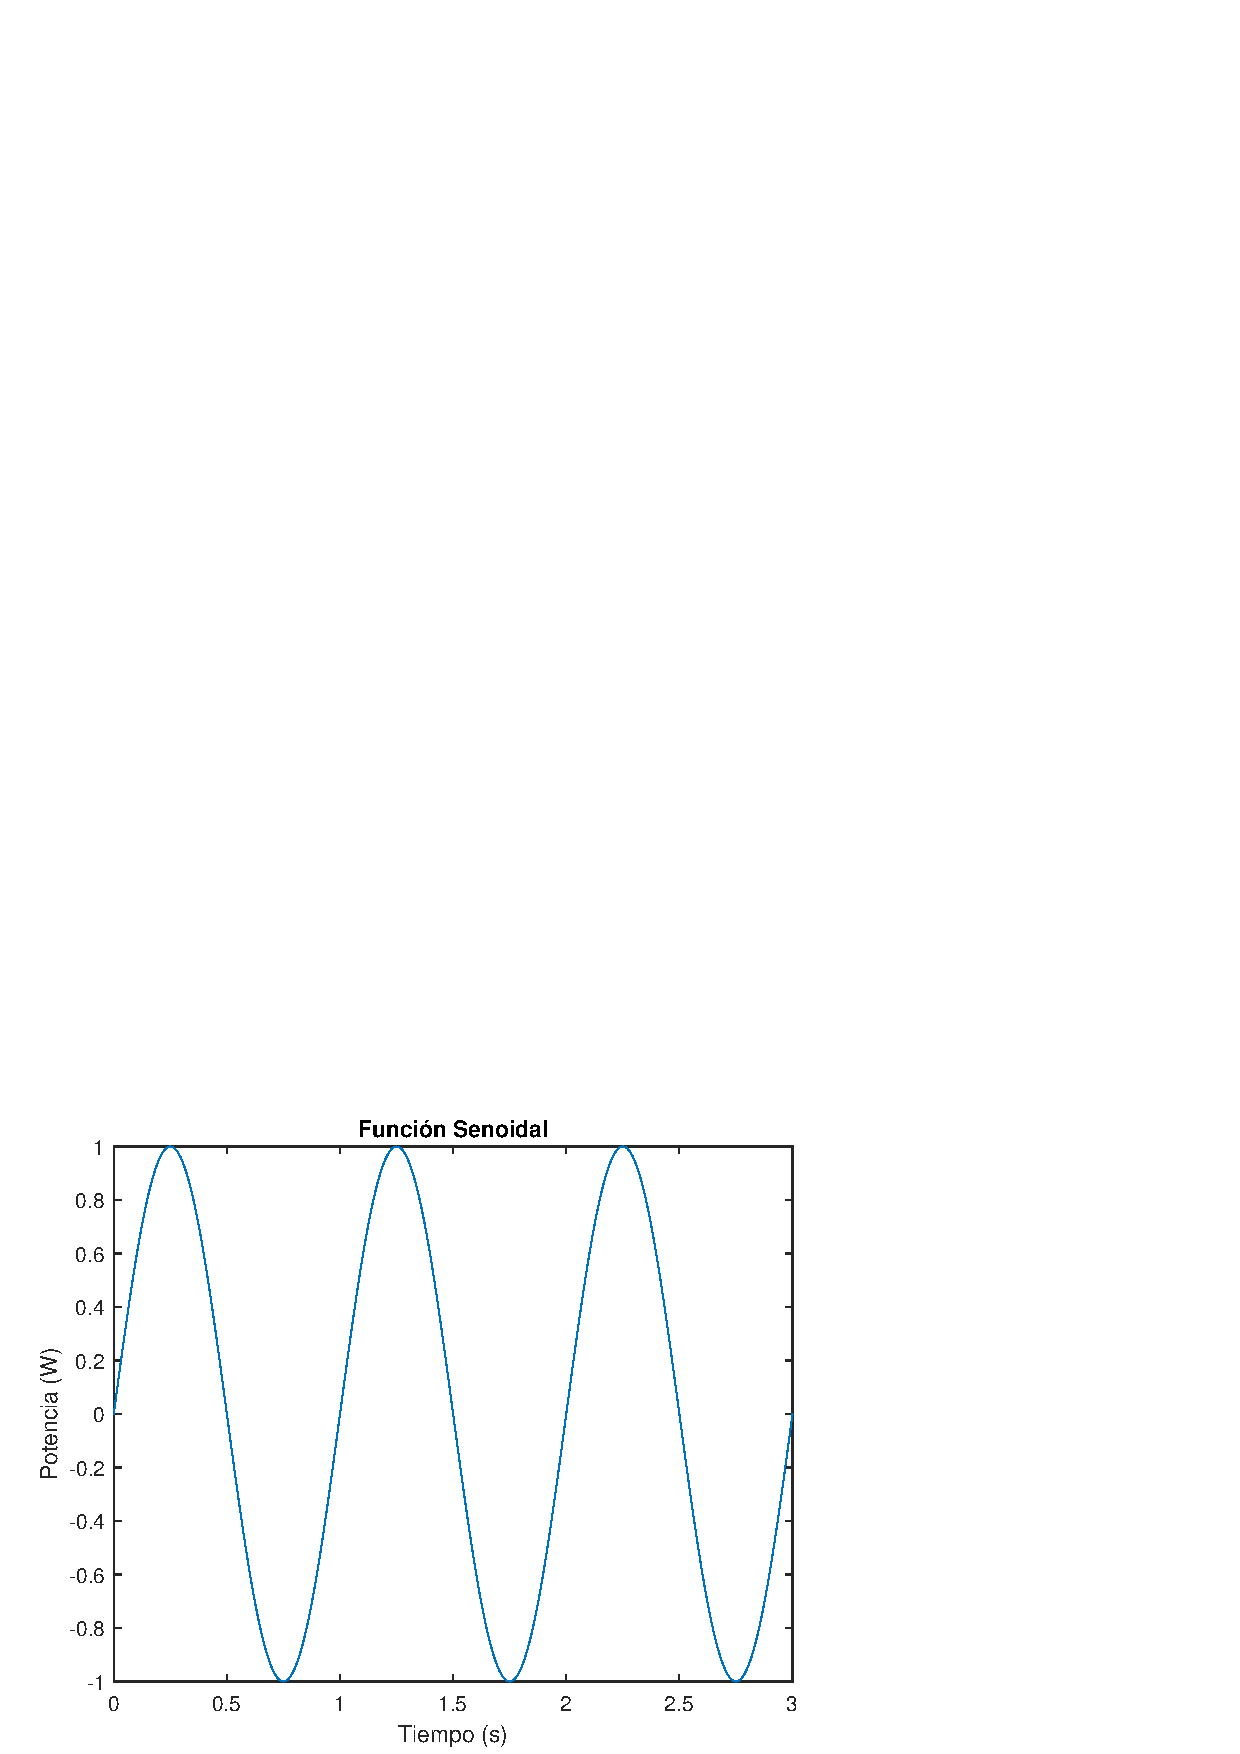
\includegraphics[width=15cm]{archivos/seno}
        \caption{Ejemplo de funcion senoidal.}
        \label{fig:seno}
\end{figure}

\par A partir de los parámetros básicos de las ondas es posible el desarrollo de otros parámetros alternativos que facilitan su comprensión y análisis como son: la longitud de onda, definida como la distancia entre los picos o valles de una onda, o el periodo, definido como el tiempo que tarda una onda en recorrer un ciclo completo. Estos dos nuevos parámetros se representan en las ecuaciones \ref{ecu:wavelength} y \ref{ecu:periodo} donde \textit{c} es la velocidad de la onda y \textit{f} la frecuencia de esta.

\begin{subequations}
	\begin{eqnarray}
		\lambda &=& \frac{c}{f} \label{ecu:wavelength} \\ % Salto de línea
		T &=& \frac{1}{f} \label{ecu:periodo}
	\end{eqnarray}
\end{subequations}

\par Pero ondas como la que se hacen referencia en la figura \ref{fig:seno}, cuyo tipo de movimiento es el movimiento armónico simple, no reflejan la realidad y la complejidad de las ondas normalmente usadas para la transmisión de información mediante \gls{oem}. Otros conceptos como la atenuación o la amortiguación han de ser tomados en cuenta para describir con mayor precisión el comportamiento de las ondas en medios de transmisión reales como el aire. Si centramos el estudio en las \gls{oem}, encargadas de transportar los mensajes en forma de energía electromagnética, se conoce que el medio en el que se propagan no tiene porqué ser necesariamente el aire, ya que estas se pueden propagar en el vacío. En este medio, las \gls{oem} se propagarán a una velocidad de 299 792 458 m/s, o más conocida como la velocidad de la luz, ya que la luz en sí es una onda electromagnética. 
\\
\par Cuando analizamos un conjunto de partículas subatómicas (electrones o protones) se puede comprobar como a sus alrededores se producen campos eléctricos debido a la interacción entre estos, de repulsión o atracción. A su vez, esta interacción en forma de movimiento de las partículas, produce un campo magnético sobre estas. Es entonces donde, la suma de ambos campos debido a las interacciones entre partículas producen campos electromagnéticos, medio donde se propagaran las \gls{oem}. \cite{Peribanez2014}
\\
\par Las \gls{oem} poseen ciertas características que las describen como son su velocidad de fase y grupo, no teniendo porqué  ser iguales, ni a su vez iguales a la velocidad de propagación en el vacío. Su vector de onda, el cual apunta la dirección en la que se dirige una onda y cuya magnitud es el número de onda. O su polarización, propiedad que aparecen en las ondas transversales como es el caso de las electromagnéticas. Por convención, cuando se habla de polarización de una \gls{oem} se hace referencia a la dirección del campo eléctrico. Existen tres tipos de polarizaciones principales: lineal, circular y elíptica, y es importante remarcar que a lo largo de este estudio todas las antenas a analizar y estudiar serán diseñadas para trabajar con polarización lineal. Si una \gls{oem} de una polarización distinta a la acordada intentara resonar en una de las antenas diseñadas, esta no llegaría a ser captada correctamente y la atenuación producida no permitiría una posible de codificación de esta. \cite{UCO}
\\
\begin{figure}[h]
    \centering
       \includegraphics[width=15cm]{archivos/oem}
        \caption{Representación esquemática de una Onda Electromagnética. \cite{Toppr2017}}
        \label{fig:oem}
\end{figure}

\par Hasta el momento solo se ha mencionado las señales como mensajes codificados en \gls{oem} que varían en el dominio temporal, pero gracias al matemático \textit{Joseph Fourier} (1768 - 1830), se pudo empezar a estudiar las ondas desde otro dominio: la frecuencia. Fourier desarrolló una serie de transformaciones matemáticas capaces de convertir las expresiones analíticas descritas en un dominio temporal a un dominio frecuencial y viceversa, a las que se denominaron como: \textit{Transformadas de Fourier}, basadas en el \textit{Teorema de Fourier} el cual señala que cualquier señal periódica puede descomponerse mediante una suma infinita de funciones de tipo sinusoidal ponderadas de forma determinada en amplitud y fase y cuyas frecuencias estén relacionadas armónicamente con la frecuencia fundamental de la onda a analizar. 
\\
\par Gracias a la Transformada de Fourier podemos analizar y sintetizar cualquier onda independientemente de su naturaleza física o matemática, y aunque no será usada como tal a lo largo de este trabajo, se hace necesario remarcar la importancia de este desarrollo matemático y la imprescindible contribución hacia el desarrollo de áreas como la acústica o las telecomunicaciones ya que todo avance realizado en esta materia tiene intrínseca la participación de la Transformada de Fourier, como es en nuestro caso, en el que toda representación de señales se realizará en el dominio frecuencial así como el hecho de poder analizar el factor de array gracias a las series de Fourier, como se verá en el capítulo~\ref{arraysdeantenas}. 
\\
\par Para terminar con el proceso de intercambio de información se hace indispensable mencionar al medio el cual puede tener dos naturalezas: guiado o radiado. El medio guiado o alámbrico es aquel que depende de una superficie conductora para transmitir la información, por lo general, un cable con propiedades conductoras como cobre u oro, pero también entran en esta categoría la fibra óptica, que transmite por sus filamentos los mensajes codificados en impulsos de luz.  
\\
\par Por otro lado tenemos el medio radiado o también denominado inalámbrico o no guiado, cuyo medio de transporte son los campos electromagnéticos. En este medio no es posible observar las ondas viajar por el espacio, exceptuando el rango de frecuencias correspondiente a la luz visible dentro del espectro electromagnético. Una de las principales propiedades de este medio es que las ondas que viajan a distinta frecuencia son inmunes entre sí a interferirse, lo que permite que los mensajes lleguen del emisor al receptor sin apenas haber sido afectadas en su trayecto por otros mensajes viajando por el campo electromagnético. A partir de ahora el papel del emisor y receptor será tomado por las antenas, las cuales serán capaces de enviar o recibir señales transmitidas en el campo electromagnético en una o varias frecuencias o longitudes de onda. Es por esto que las antenas quedan ahora como los elementos claves para la transmisión de información inalámbrica. 
\\ 
\par En la actualidad existen varios tipos de antenas, como estudiaremos más detenidamente en el capítulo \ref{antenasmicrostrip} y cada uno de ellas se adaptará más específicamente a nuestras necesidades de directividad, ganancia, ancho de banda o eficiencia entre otros. En el estudio que se va a realizar, se diseñarán una serie de  arrays de parches en tecnología microstrip que será capaz de trabajar a las frecuencias especificadas para la \gls{5g} de comunicaciones móviles por el \gls{3gpp} así como otras tecnologías como Wi-Fi o Bluetooth.

\section{Las comunicaciones móviles}
\subsection{Las primeras generaciones de telefonía}
\par Las comunicaciones inalámbricas han supuesto una revolución desde su aparición a finales del siglo XX hasta la actualidad. El avance de la tecnología, la miniaturización de los componentes, la necesidad de comunicación internacional e incluso las competencias económicas han sido factores claves en la evolución de las comunicaciones móviles. Al hablar de comunicaciones móviles se incluyen en su espectro desde aquellas primeras comunicaciones analógicas como el \textit{Walkie Talkie} o la \gls{1g} hasta los métodos actuales más avanzados como la \gls{4glte}, comunicaciones vía satélite o \gls{voip}. Si se estrecha el círculo al ámbito de la telefonía móvil se puede observar como desde los años 80 distintos estándares de comunicaciones móviles han sido adoptados de la mano de la tecnología disponible en la época e incluso obligando a esta a mejorar para conseguir unos mejores resultados sobre el estándar. 
\\
\par El \gls{1g} fue el primer estándar de telefonía móvil. Fue lanzado en 1979 por la \gls{ntt} en Japón, donde rápidamente se extendió su uso desde su comienzo en el área metropolitana de Tokyo hasta cubrir por completo el área de la isla. Dos años más tarde en 1981 la \gls{nmt} empezó a desplegar esta red en países como Finlandia, Dinamarca o Noruega y más tarde extendiéndose hasta Rusia bajo su propio estándar. En Estados Unidos y Australia esta generación se desplegó bajo el estándar \gls{amps} desarrollado por Motorola y en Reino Unido como \gls{tacs}. \cite{Wikipedia}
\\
\par En España la \gls{ctne} actualmente conocida como Telefónica, desplegó, bajo el servicio MoviLine, su oferta de \gls{1g} mediante el estándar ETACS, una actualización del sistema \gls{tacs} que incluía una nueva banda de frecuencias. Esta primera generación de telefonía móvil se basaba en el uso de la electrónica sólo en los servicios de red de acceso, ya que el resto de la red de comunicación se sostenía sobre la red analógica de telefonía ya existente en cada país, con lo que solo se permitía el tráfico de voz sobre ella. \cite{Wikipediaa}

\begin{figure}[h]
    \centering
        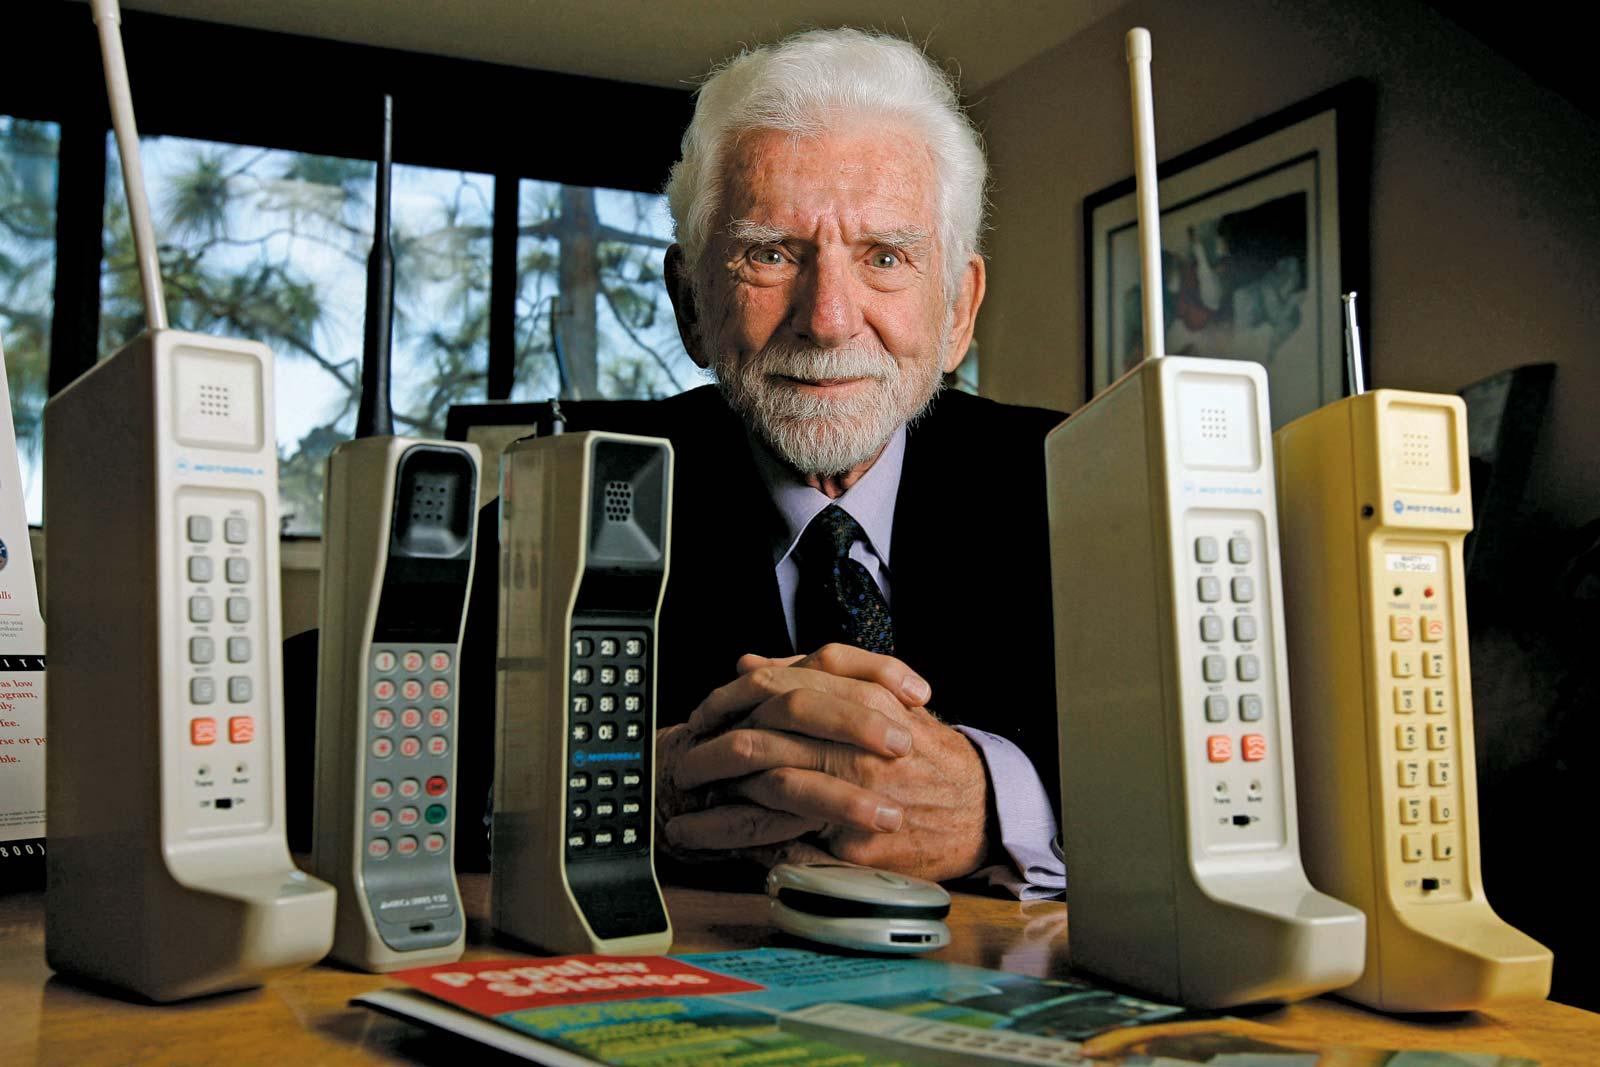
\includegraphics[width=15cm]{archivos/motorola}
        \caption{Martin Cooper (Motorola) junto a teléfonos móviles de primera generación. \cite{Huffaker2009}}
        \label{fig:motorola}
\end{figure}

\par Tras una década, en el año 1992, apareció el siguiente estándar de telefonía, la \gls{2g}, donde se adoptaron sistemas digitales tanto en la red de acceso o \gls{ran}, como en el Core, es decir la parte central de la red de telecomunicaciones donde, entre otras funcionalidades, se enruta el tráfico.
El estándar asociado al \gls{2g} fue el denominado \gls{gsm}, este era capaz de, además de realizar llamadas, ahora sí sobre la red digital, la transmisión de paquetes de datos, lo que permitió el uso de mensajería instantánea con el SMS o las primeras conexiones a Internet móvil, aun más consolidado con la evolución del estándar \gls{gsm}: el \gls{gprs}, que conseguía throughputs, o tasas de transmisión efectivas de hasta 230 Kbps en su último release (EDGE), también conocido como el 2.5G. \cite{LaCuevaGSM2014} 
\\
\par Esta generación de telefonía móvil se desplegó sobre las bandas de 900 y 1800 Mhz. En España, tras la desaparición del servicio MoviLine, apareció Movistar, también bajo el mando de Telefónica, con el primer despliegue de red digital móvil. Tras la liberación del mercado de las telecomunicaciones, otras operadoras como Airtel (Vodafone) o Amena (Orange) empezaron a ofrecer sus servicios móviles a nivel nacional. \cite{Wikipedia2019b}
\\
\par Otra de las novedades del estándar \gls{2g} fue la incursión de la denominada Tarjeta SIM, la cual permitía identificar a cada suscriptor. En su interior era capaz de almacenar la información sobre la suscripción del usuario, un directorio telefónico o los parámetros de la red a la que se debía conectar según la operadora. Actualmente la mayoría de países que adoptaron esta tecnología están en proceso de desconexión de sus estaciones bases \gls{2g} puesto que se considera un estándar ya obsoleto y su uso ha quedado restringido a ciertas zonas donde las operadoras no consideraron conveniente el despliegue de nuevas redes de telefonía como en zonas rurales o carreteras. \cite{Wikipedia2019b}
\subsection{La tercera generación}
\par A principios de este siglo, la \gls{3g} de telefonía fue lanzada por la \gls{itu} bajo el nombre de IMT-2000. A esta generación de telefonía también se le denominó \gls{umts}, y es que es el primer estándar que aseguraba compatibilidad telefónica entre países ya que el consorcio encargado de velar por el correcto uso del estándar, la \gls{3gpp}, estaba formado por empresas tecnológicas internacionales como \gls{att}, Ericsson, Motorola o \gls{ntt}. Este nuevo servicio de telefonía permitía conectividades de hasta 20 Mbps en su banda de 2100 MHz, lo que permitió la proliferación de los \textit{smartphones}, donde ahora ya era posible acceder fácilmente a Internet, el correo electrónico u otros servicios multimedia online. \cite{LaCuevaGSM2014, Wikipedia2019} 
\\
\par El \gls{3g} implementaba un nuevo tipo de modulación denominada \gls{wcdma}, el cual permitía una mayor eficiencia espectral debido a que todos los usuarios eran capaces de transmitir simultáneamente, pero separados mediante códigos de identificación únicos. Para separar la señal en el medio de transmisión cada bit era multiplicado por el código de identificación de cada usuario. Conforme pasaron los años, nuevos sub-estándares fueron lanzados mejorando las especificaciones iniciales del \gls{3g}, como el \gls{hspa}, que permitía tasas de transmisión de hasta 42 Mbps y 168 Mbps en HSPA+ e introducía por primera vez los conceptos de \gls{mimo} y \textit{beamforming} que se explicarán más adelante.


\subsection{Actualidad, la cuarta generación}
\par Finalmente, en el año 2013 se lanzó oficialmente el \gls{4glte}, desarrollado también por el \gls{3gpp}. El término LTE, en español, ``evolución a largo plazo" es adoptado para este estándar puesto que realmente esta generación no añade una arquitectura nueva al sistema sino que se basa en las arquitecturas ya consolidades del \gls {3g} y el \gls{2g}. Es por esto que la \gls{itu} no consideró que el LTE desplegado actualmente sea una completa nueva generación, en este caso \gls{4g}. Las principales características del \gls{lte} son un incremento de las tasas de transmisión, una mayor eficiencia energética y seguridad, una menor latencia, y más fácil de desplegar por los operadores. \cite{LaCuevaGSM2014, Zavias2012}
\\
\par Con el \gls{lte} se han llegado a conseguir tasas de hasta 173 Mbps de bajada, y con la implementación de \gls{mimo} con 4 antenas en los dispositivos, esta se duplicaba hasta los 300 Mbps. Además, en este nuevo estándar, sólo se utiliza la conmutación de paquetes, es decir, se descartaban por completo en el Core de la red, los antiguos sistemas de conmutación de circuitos para transferir las llamadas. La modulación escogida para el \gls{lte} fue la \gls{ofdm}, la cual transporta la información modulada en \gls{qam} pero multiplexado en un conjunto de diferentes portadoras, lo que permite una mayor eficiencia espectral con respecto al \gls{3g}.
\subsection{El futuro, la quinta generación}
\par El \gls{5g} es el nuevo estándar de telefonía móvil, sucesora de la \gls{4g}, llevado a cabo por el \gls{3gpp} en su Release 15 y 16. Este nuevo estándar de telefonía permitirá: \cite{3GPP2019, Gemalto2019, MINECO2019}
\\
\begin{itemize}
\item Conexiones con throughputs, o tasas de transmisión efectivas de hasta 10 Gbps, es decir, hasta 10 veces más rápido que el \gls{4g}.
\item La latencia, definida como la suma de retrasos temporales producidas en un sistema de comunicación debido a la velocidad de propagación limitada, perdidas, etc. se reducirán hasta valores de 1 ms en comparación con el rango de entre 30 y 50 ms que obtenemos en redes \gls{4g} y Wi-Fi.
\item Capacidad de conexiones masivas para dispositivos \gls{iot}, lo que permitirá  el desarrollo de redes de comunicación \gls{m2m} aumentando la eficiencia energética de estas, así como su disponibilidad y seguridad, lo que será imprescindible para tecnologías emergentes como la conducción autónoma o las Smart Cities, es decir, el proceso de uso de las \gls{tic} para modernizar el entorno urbano ofreciendo servicios de mejora del transporte público, seguridad ciudadana, ahorro energético, etc.
\item Mejora de la diversidad en recepción con respecto al \gls{4g} mediante el uso del \gls{mimo} Masivo. Esta tecnología aprovecha el uso de múltiples antenas sobre un mismo dispositivo para usarlas como enlaces independientes, de forma que la velocidad de conexión pueda aumentar de forma significativa. Con \gls{mmimo} se dispondrán de decenas de antenas por dispositivo para hacer que la conexión sea más rápida y eficiente.
\item El uso de \textit{beamforming}, proceso por el cual se direcciona el haz de emisión de la antena y mediante técnicas de procesado digital se calcula en qué dirección se hará más eficiente la comunicación entre la antena y el dispositivo además de poder hacer cálculos sobre ruido e interferencias para mejorar la eficiencia de la antena.
\end{itemize}

\par Además, el \gls{5g} emitirá sobre nuevas bandas de frecuencia, las cuales categorizaremos como \textit{Bandas Sub-6GHz} y \textit{Bandas Super-6GHz}. En el caso del plan nacional para el 5G aprobado por el \gls{minetur}, principal responsable de la gestión de los temas referentes a telecomunicaciones a nivel estatal en España, las bandas de frecuencias aprobadas para el 5G son:
\\
\begin{itemize}
\item\textbf{700 Mhz:} esta banda antes usada para la retransmisión de la \gls{tdt} y adjudicada para su uso en el \gls{5g} mediante el segundo dividendo digital \cite{MINECO2019a} será clave para la retransmisión de señales móviles \gls{5g} que necesitan alcanzar los interiores de los hogares y las oficinas puesto que su mayor longitud de onda con respecto a otras bandas la hace apta para penetrar o difractar sobre muros.
\item\textbf{3.4-3.8 GHz: }estas bandas de frecuencias eran anteriormente usadas para radioenlaces de transporte de señal de televisión, actualmente en desuso. Permitirán mayores tasas de velocidad con respecto a los 700 Mhz, pero su atenuación será mayor, lo que la hace adecuada para transmisión en zonas urbanas o carreteras.
\item\textbf{27 GHz: }en este rango de frecuencias entramos en las denominadas como \gls{mmwv} es decir, ondas cuya longitud de onda esté en el orden de milímetros. Esta banda de frecuencia presume de tener mayor disponibilidad en cuanto a ancho de banda lo que permitirá conexiones de banda ancha ultra rápidas.
\end{itemize}

\par Como se puede ver, la tendencia futura en cuanto a comunicaciones móviles de alta velocidad va de la mano y es directamente proporcional a la frecuencia a la que se emita la señal, pero a su vez, este incremento de frecuencia hace más vulnerables a las transmisiones de ser interferidas o atenuadas durante su transmisión, lo que haría muy difícil el uso de las redes \gls{5g} cuando la antena se sitúa en el exterior y los dispositivos en interiores. En este escenario surge el concepto, ya existente en el \gls{4g} del uso de \textit{Small Cells}. Las \textit{Small Cells} son pequeñas estaciones base que se sitúan en puntos estratégicos tanto en interiores como oficinas o centros comerciales, como en exteriores en sitios con una gran afluencia de personas y por ende, de dispositivos móviles. 
\\
\par En el \gls{5g}, el concepto de \textit{Small Cell} (fig. \ref{fig:stadika}) es imprescindible. Debido al crecimiento exponencial del uso de dispositivos por parte de usuarios y empresas cada vez se hará más difícil el hecho de que una sola estación base pueda dar cobertura y una tasa de transmisión aceptables al estándar a estos dispositivos. Es por ello que en los nuevos despliegues de \gls{5g} las operadoras se inclinarán más por el uso de muchas \textit{Small Cells} a lo largo de la ciudad que den servicio a los usuarios de un rango muy limitado de espacio, pero con muy buena cobertura y tasas de transmisión, que a la instalación de estaciones base convencionales que dan cobertura en radios muy amplios de distancia, lo que en grandes urbes puede suponer la saturación de la propia estación base.
\\
\begin{figure}[h]
    \centering
        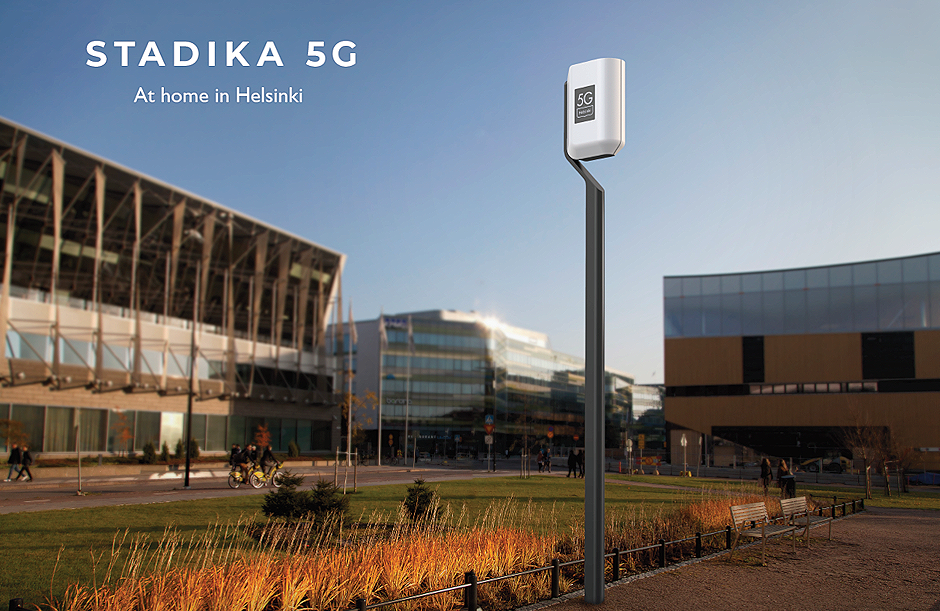
\includegraphics[width=\textwidth]{archivos/stadika}
        \caption{Stadika: concepto de diseño de Small Cells 5G para la ciudad de Helsinki. \cite{Muesa2019}}
        \label{fig:stadika}
\end{figure}

\par Bajo todo este nuevo escenario de comunicaciones avanzadas que plantea para un futuro muy cercano se han de plantear qué tecnologías se usarán para cubrir las metas y especificaciones marcadas de la manera más robusta y eficiente. El \gls{5g} tendrá una completa dependencia de los sistemas informáticos diseñados para alcanzar estas metas, mediante técnicas de procesado digital y nuevos algoritmos podremos ir añadiendo características e incluso mejorando las ya existentes sin necesidad de alterar todo el sistema ya instalado en la red.

\section{Motivación}
\par Ante todo este nuevo escenario de tecnología móvil que se plantea para los próximos años cabe la necesidad de adaptar la tecnología existente para ser compatible con las nuevas especificaciones. En el fondo la pieza clave de toda comunicación inalámbrica digital es la antena, y es importante que un correcto diseño de esta para asegurar que los parámetros de funcionamiento de están aseguren una correcta adaptación al estándar. 
\\
\par Las antenas de parche de tipo microstrip llevan siendo usadas durante décadas para la transmisión de información entre dispositivos móviles y las estaciones base, así como en comunicaciones aéreas, satelitales, o aeroespaciales, debido a la flexibilidad respecto a su tamaño, peso, coste, rendimiento e incluso facilidad de instalación. En este proyecto se diseñarán y analizarán una serie de arrays o conjunto de antenas, que permitirán mejorar ciertas características del sistema, para trabajar a las frecuencias de 2.4, 6, e incluso 27 GHz. 
\\
\par La banda de 2.4 GHz es actualmente usada por las comunicaciones \gls{wifi} comerciales, y servirá para dar una idea sobre los conceptos básicos de diseño de antenas microstrip así como servir de comparativa para las otras configuraciones. La banda de 6 GHz aunque actualmente no está licitada para el uso de la tecnología \gls{5g} se trata de una banda con un gran potencial, que podrá proveer a los dispositivos de velocidades por encima de estándares \gls{wifi} IEEE 802.11ac pero con cobertura limitada. El uso comercial de esta banda está siendo estudiado por diferentes países para la futura incorporación al estándar \gls{5g} \cite{5GAmericas2019}. Finalmente, la banda de 27 GHz ya está licitada para su uso en Europa para el estándar \gls{5g} y con ella se prevé obtener velocidades de hasta varios gigabits, y pocas unidades de milisegundos de latencia, lo que abre las puertas a aplicaciones que requieran conexiones de latencia cero hasta ahora vetadas por la propia tecnología.


\section{Estructura del proyecto y metodología}
\label{sec:medodologia}
\par Este proyecto estará dividido en dos partes fundamentales, un marco teórico, donde se realizará un completo resumen sobre los conceptos básicos de las líneas de transmisión: adaptación e impedancias, tecnología microstrip en líneas de transmisión, etc. Antenas: tipos de antena, parámetros de estudio básicos, etc. Y en un marco más específico, sobre las antenas de tipo parche en tecnología microstrip: métodos de alimentación, componentes, tipos, análisis, etc. Finalmente se expondrá la parte de experimentación, donde se estudiarán y analizarán los diseños de distintos tipos de configuraciones de arrays para antenas de tipo parche con tecnología microstrip.
\\
\par Para realizar la parte experimental del proyecto se hará uso del software de análisis electromagnético 3D: Ansys\textregistered HFSS (High Frequency Structure Simulator). Este software es usado para diseñar y simular componentes electrónicos de alta frecuencia como antenas, arrays, filtros o placas de circuito impreso. Con él, se diseñarán las configuraciones de antenas especificadas y se simularán sus efectos electromagnéticos como si se tratara de una cámara anecóica, para finalmente poder analizar los resultados obtenidos y los valores de los parámetros característicos de la antena así como comprobar la viabilidad del producto final en términos de rendimiento o dimensiones.
\\
\par Por otro lado, se hará uso de la herramienta de cálculo matemático MathWorks\textregistered MATLAB, con la que realizaremos cálculos básicos sobre las dimensiones de la antena a diseñar en función a los parámetros de construcción de esta.
